\subsection{Separation of boundary layers (64-65)}

Boundary condition at the wall:
\begin{equation}
v_x(x,y=0) = v_y(x,y=0)=0
\end{equation}

Prandtl equation (with pressure)
\begin{equation}
v_x\pdiff{v_x}{x}+v_y\pdiff{v_x}{y} = -\frac{1}{\rho_0}\pdiff{p}{x}+\frac{\mu}{\rho_0}\ppdiff{v_x}{y}
\end{equation}
If we are very close to the wall, the two terms on the left side equal zero. We then have
\begin{equation}
\pdiff{p(x,y=0)}{x}=\mu\ppdiff{v_x(x,y=0)}{y}
\end{equation}

\begin{figure}[!h]
    \centering
    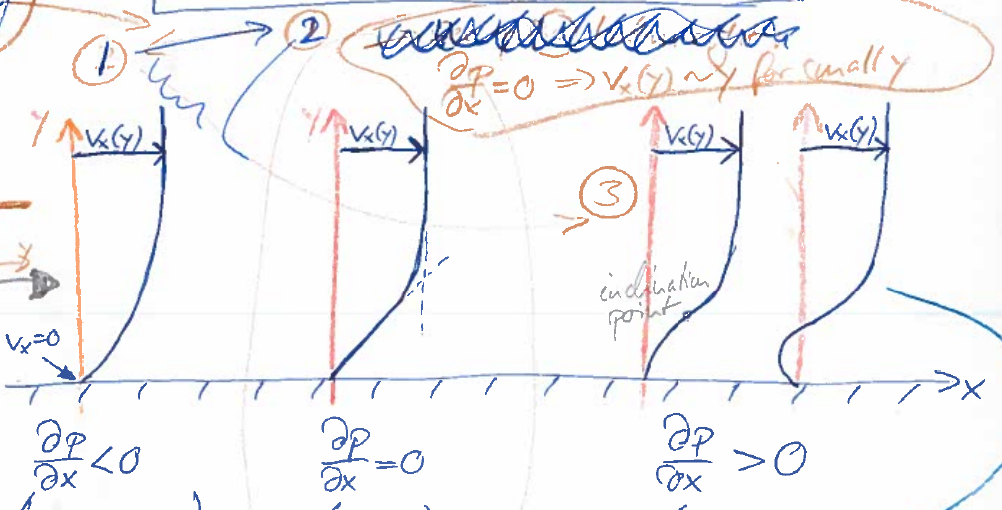
\includegraphics[width=.9\textwidth]{week5/wall-boundary}\\
    \caption{}
    \label{fig:wall-boundary}
\end{figure}

\begin{figure}[!h]
    \centering
    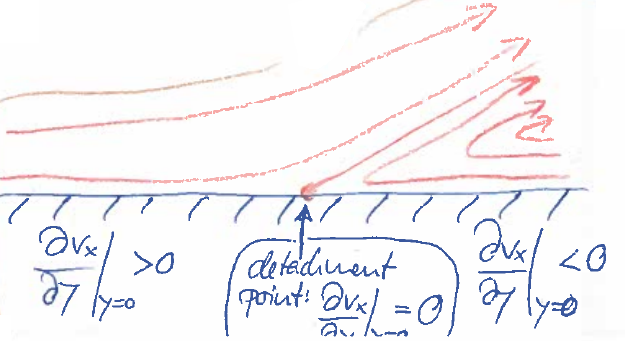
\includegraphics[width=.5\textwidth]{week5/detachment-point}\\
    \caption{}
    \label{fig:detachment-point}
\end{figure}

\newpage
\textbf{Example:} flow around cylinder

\begin{figure}[!h]
    \centering
    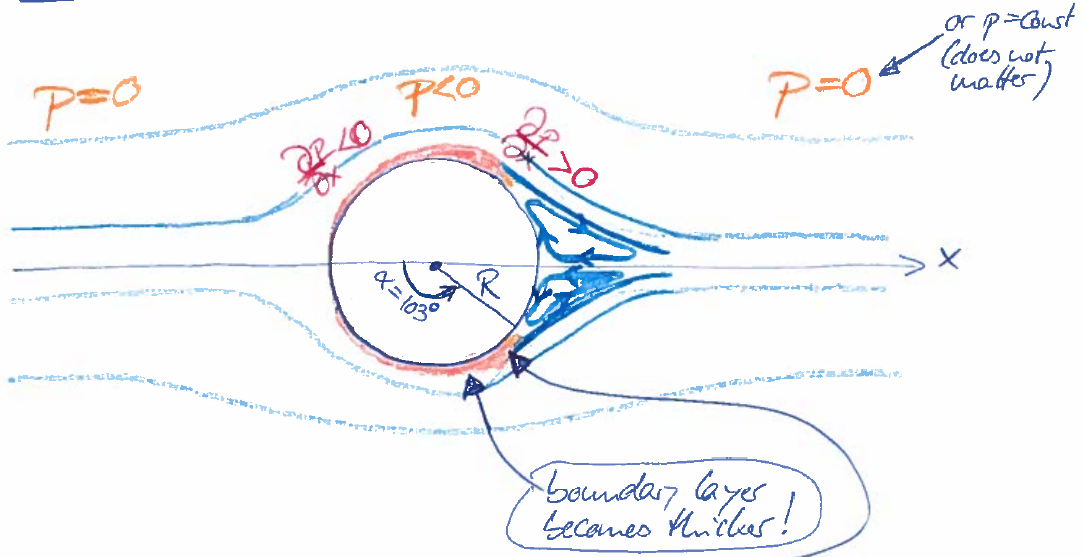
\includegraphics[width=.8\textwidth]{week5/cylinder-flow}\\
    \caption{}
    \label{fig:cylinder-flow}
\end{figure}

The detachment point is at the separation of the boundary layer. When $v\approx0$ there is no kinetic energy to run against the pressure gradient.

\begin{framed}
\textbf{Remark:} separation of boudnary layers is a big issue in mechanical engineering; for example: design of airfoils, wind-turbine blades etc.
{\center
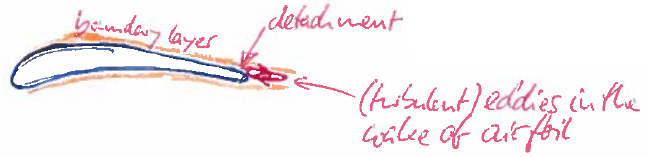
\includegraphics[width=.4\textwidth]{week5/detachment-eddies}\\
}
In case of separation the lift decreases, which can lead to airplane crash. It would also lead to a substantial rise in the overall drag (more friction). This would require more engine power and therefore more fuel for an airplane. For a wind turbine it would means less power generation.

Engineer's dream: construct airfoils without turbulent wake to mimic shark skin or fish scales.
\end{framed}

\subsection{Solution of Prandtl equations for free boundary layers (66-71)} 

\fref{fig:2d-laminar-jet} shows a 2-dimensional laminar jet flow generated from a flow through a long slit streaming into a resting fluid.

\begin{figure}[!h]
    \centering
    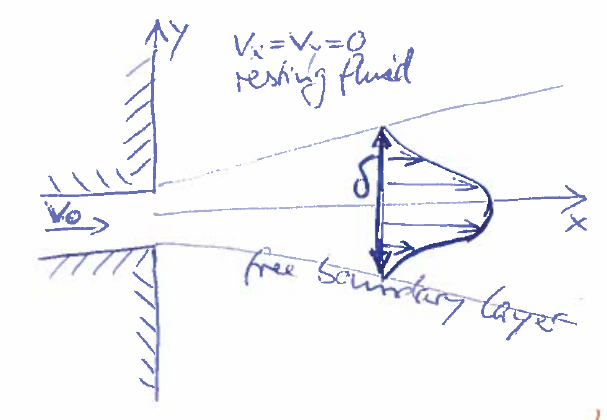
\includegraphics[width=.6\textwidth]{week5/2d-laminar-jet}\\
    \caption{}
    \label{fig:2d-laminar-jet}
\end{figure}

We use the Prandtl equations with the similarity ansatz:
\begin{equation}
v_x(x,y)=v_\mathrm{max}(x)g\left(\frac{y}{\delta(x)}\right)
\end{equation}

\begin{equation}
\pdiff{v_x}{x}+\pdiff{v_y}{y}=0 \Rightarrow v_x=\pdiff{\psi}{y},\quad v_y=-\pdiff{\psi}{x}
\end{equation}

\begin{equation}
\psi = v_\mathrm{max}(x)\delta(x)f\left(\frac{y}{\delta(x)}\right)
\end{equation}

\begin{equation}
\pdiff{\psi}{y}=v_\mathrm{max}\delta f'\frac{1}{\delta}=v_\mathrm{max}f'=v_\mathrm{max}g=v_x
\end{equation}

\begin{equation}
v_y=-\pdiff{\psi}{x}=-v'_\mathrm{max}\delta f-v_\mathrm{max}\delta'f-v_\mathrm{max}\delta f'\frac{(-y)\delta'}{\delta^2}
\end{equation}

\begin{align}
\partial_xv_x &= v'_\mathrm{max}f'+v_\mathrm{max}f''\frac{(-y)\delta'}{\delta^2} \\
\partial_yv_x &= v_\mathrm{max} f''\frac{1}{\delta}\\
\partial^2_xv_x &= \frac{v_\mathrm{max}}{\delta^2}f'''
\end{align}

\begin{align}
\begin{split}
v_x\partial_x v_x+v_y\partial_yv_x-\frac{\mu}{\rho_0}\partial^2_yv_x &= v_\mathrm{max}f'\left\lbrace v'_\mathrm{max}f' - v_\mathrm{max}\frac{y\delta'}{\delta^2}f''\right\rbrace \\
&\hspace{5mm}-\left\lbrace v'_\mathrm{max}\delta f + v_\mathrm{max}d'f-v_\mathrm{max}\frac{y\delta'}{\delta}f'\right\rbrace v_\mathrm{max}\frac{1}{\delta}f'' \\
&\hspace{5mm}-\frac{\mu}{\rho_0^2} \frac{v_\mathrm{max}}{\delta^2}f'''
\end{split}\\
\begin{split}
&= v_\mathrm{max}v'_\mathrm{max}f'^2-v_\mathrm{max}v'_\mathrm{max}ff''-v_\mathrm{max}^2\frac{\delta'}{\delta}ff'' \\
&\hspace{5mm}-\frac{\mu}{\rho_0}\frac{v_\mathrm{max}}{\delta^2}f'''\label{eq:free-boundary}
\end{split} \\
&\require0
\end{align}
All four terms in \eqref{eq:free-boundary} have the form $\alpha_i(x)\beta_i(x)$ for $(i=1,...,4)$. The sum of these four terms has to be zero. This means that $\alpha_1(x)\sim\alpha_2(x)\sim\alpha_3(x)\sim\alpha_4(x)$.

Ansatz:
\begin{align}
v_\mathrm{max}(x) &= c_1x^m\\
\delta(x) &= c_2 x^n
\end{align}

\begin{framed}
\textbf{Remark:} we expect $m<0$ (decreasing velocity with penetration depth) and $n>0$ (increasing thickness of jet with penetration depth).
\end{framed}

Sum of the 4 terms:
\begin{equation}
c_1^2mx^{2m-1}(f'^2-ff'')-c_1^2x^{2m}\frac{n}{x}ff'' - \frac{\mu}{\rho_0}\frac{c_1}{c_2^2}\frac{x^m}{x^{2n}}f'''=0
\end{equation}

\begin{equation}
2m-1 = m-2n
\end{equation}

\begin{equation}
m(f'^2-ff'')nff''-\frac{\mu}{\rho_0}\frac{1}{c_1c_2^2}f'''=0
\end{equation}
This differential equation determines the velocity profile
\begin{equation}
g\left(\frac{y}{\delta(x)}\right)=f'\left(\frac{y}{\delta(x)}\right)
\end{equation}
of the jet. We are not going to solve this, but we want to know $m$ and $n$, because they determine $v_\mathrm{max}(x)$ and $\delta(x)$. We need a second equation for $m$ and $n$.

\textbf{Second equation:} conservation of momentum flux.
Momentum flux through the red plane in \fref{fig:momentum-flux} is identical to the momentum flux through the blue plane. This means that the integrated momentum flux does not depend on $x$.
\begin{figure}[!h]
    \centering
    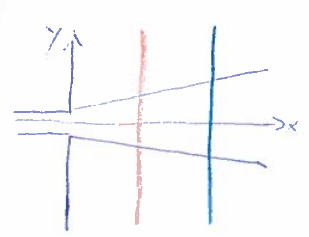
\includegraphics[width=.4\textwidth]{week5/momentum-flux}\\
    \caption{}
    \label{fig:momentum-flux}
\end{figure}

\begin{align}
\mathrm{momentum} & =\rho_0\Delta V\cdot v_x\\
&= \rho_0\Delta Av_x\Delta tv_x
\end{align}

Momentum flux:
\begin{equation}
\frac{\mathrm{momentum}}{\Delta A \Delta t} = \rho_0 v_x^2
\end{equation}

\noindent\makebox[\linewidth]{\rule{\textwidth}{0.5pt}}
\textbf{Proof of conservation of momentum flux}

If
\begin{equation}
\int_{-\infty}^\infty \rho_0v_x^2(x)dy=\mathrm{constant}
\end{equation}
then
\begin{equation}
\diff{}{x}\int_{-\infty}^\infty \rho_0v_x^2(x)dy=0
\end{equation}

\begin{align}
\diff{}{x}\int_{-\infty}^\infty \rho_0v_x^2(x)dy &= 2\rho_0\int_
{-\infty}^\infty\left(v_x\pdiff{v_x}{x}\right)dy \\
&= 2\mu\pdiff{v_x}{y}\biggm\vert_{-\infty}^\infty-2\rho_0\int_{-\infty}^\infty v_y\pdiff{v_x}{y}dy \\
&=-2\rho_0v_xv_y\biggm\vert_{-\infty}^\infty + 2\rho_0 \int_{-\infty}^\infty\pdiff{v_y}{y}dy \\
&= -2\rho_0\int_{-\infty}^\infty v_x\pdiff{v_x}{x}dy\\
&= 0
\end{align}
\noindent\makebox[\linewidth]{\rule{\textwidth}{0.5pt}}

\begin{align}
\int_{-\infty}^\infty\rho_0v_x^2dy &= \rho_0\int_{-\infty}^\infty v_\mathrm{max}^2(x)g^2\left(\frac{y}{\delta(x)}\right)dy\\
&= \rho_0v_\mathrm{max}^2(x)\delta(x)\int_{-\infty}^\infty g^2(z)dz\\
&\require \mathrm{constant}
\end{align}

\begin{align}
v_\mathrm{max}^2(x)\delta(x)&=\mathrm{constant}\\
c_1^2x^{2m}c_2x^n &= \mathrm{constant}\\
2m+n&0
\end{align}

\begin{align}
m+2n=1\ &,\qquad 2m+n=0 \\
\leadsto
m=-\frac{1}{3}\ &,\qquad n=\frac{2}{3}
\end{align}

\begin{align}
v_\mathrm{max}(x)&\sim\frac{1}{x^{1/3}}\\
\delta(x)&\sim x^{2/3}
\end{align}

\begin{framed}
\textbf{Remark:} negative jet flow

Wake behind a wind turbine can be modeled as a negative jet.

{\center
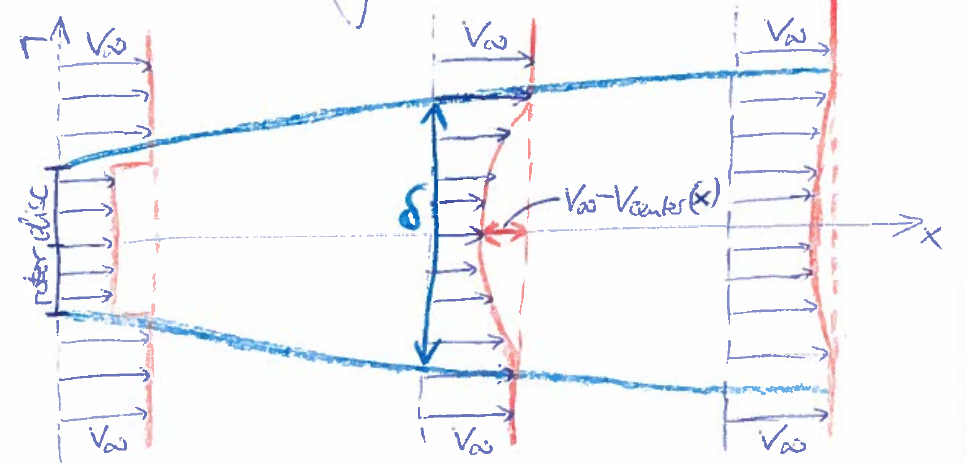
\includegraphics[width=.7\textwidth]{week5/negative-jet}\\
}

\begin{equation}
v_x(x,r) = v_\infty-v_\mathrm{center}(x)g\left(\frac{r}{\delta(x)}\right)
\end{equation}
\end{framed}